\documentclass[10pt,twocolumn]{article}
% Shared two-column preamble for the three research papers.
% Use with: \documentclass[10pt,twocolumn]{article}
% Then in main.tex: % Shared two-column preamble for the three research papers.
% Use with: \documentclass[10pt,twocolumn]{article}
% Then in main.tex: % Shared two-column preamble for the three research papers.
% Use with: \documentclass[10pt,twocolumn]{article}
% Then in main.tex: \input{../../shared/latex/twocolumn_preamble.tex}

\usepackage[margin=0.75in]{geometry}
\usepackage[utf8]{inputenc}
\usepackage[T1]{fontenc}
\usepackage{lmodern}
\usepackage{microtype}
\usepackage{amsmath,amssymb,amsthm}
\usepackage{graphicx}
\usepackage{booktabs}
\usepackage{caption}
\usepackage{subcaption}
\usepackage{hyperref}
\usepackage{url}
\usepackage{xcolor}
\usepackage{algorithm}
\usepackage{algorithmic}
\usepackage{multirow}
\usepackage{titlesec}
\usepackage{authblk}

\hypersetup{colorlinks=true,linkcolor=blue!50!black,citecolor=blue!50!black,urlcolor=blue!50!black}

\titleformat{\section}{\normalfont\large\bfseries}{\thesection}{0.6em}{}
\titleformat{\subsection}{\normalfont\bfseries}{\thesubsection}{0.5em}{}

\captionsetup{font=small,labelfont=bf,skip=4pt}
\setlength{\columnsep}{0.25in}
\setlength{\parskip}{2pt}

\newtheorem{theorem}{Theorem}
\newtheorem{proposition}[theorem]{Proposition}
\newtheorem{definition}[theorem]{Definition}


\usepackage[margin=0.75in]{geometry}
\usepackage[utf8]{inputenc}
\usepackage[T1]{fontenc}
\usepackage{lmodern}
\usepackage{microtype}
\usepackage{amsmath,amssymb,amsthm}
\usepackage{graphicx}
\usepackage{booktabs}
\usepackage{caption}
\usepackage{subcaption}
\usepackage{hyperref}
\usepackage{url}
\usepackage{xcolor}
\usepackage{algorithm}
\usepackage{algorithmic}
\usepackage{multirow}
\usepackage{titlesec}
\usepackage{authblk}

\hypersetup{colorlinks=true,linkcolor=blue!50!black,citecolor=blue!50!black,urlcolor=blue!50!black}

\titleformat{\section}{\normalfont\large\bfseries}{\thesection}{0.6em}{}
\titleformat{\subsection}{\normalfont\bfseries}{\thesubsection}{0.5em}{}

\captionsetup{font=small,labelfont=bf,skip=4pt}
\setlength{\columnsep}{0.25in}
\setlength{\parskip}{2pt}

\newtheorem{theorem}{Theorem}
\newtheorem{proposition}[theorem]{Proposition}
\newtheorem{definition}[theorem]{Definition}


\usepackage[margin=0.75in]{geometry}
\usepackage[utf8]{inputenc}
\usepackage[T1]{fontenc}
\usepackage{lmodern}
\usepackage{microtype}
\usepackage{amsmath,amssymb,amsthm}
\usepackage{graphicx}
\usepackage{booktabs}
\usepackage{caption}
\usepackage{subcaption}
\usepackage{hyperref}
\usepackage{url}
\usepackage{xcolor}
\usepackage{algorithm}
\usepackage{algorithmic}
\usepackage{multirow}
\usepackage{titlesec}
\usepackage{authblk}

\hypersetup{colorlinks=true,linkcolor=blue!50!black,citecolor=blue!50!black,urlcolor=blue!50!black}

\titleformat{\section}{\normalfont\large\bfseries}{\thesection}{0.6em}{}
\titleformat{\subsection}{\normalfont\bfseries}{\thesubsection}{0.5em}{}

\captionsetup{font=small,labelfont=bf,skip=4pt}
\setlength{\columnsep}{0.25in}
\setlength{\parskip}{2pt}

\newtheorem{theorem}{Theorem}
\newtheorem{proposition}[theorem]{Proposition}
\newtheorem{definition}[theorem]{Definition}

\newcommand{\gptTwoProbeEnPeak}{1.000}
\newcommand{\gptTwoProbeClPeak}{0.959}
\newcommand{\gptTwoCrossEnCl}{0.669}
\newcommand{\gptTwoCrossClEn}{0.594}
\newcommand{\gptTwoProbeEnPeakLayer}{6}
\newcommand{\gptTwoProbeClPeakLayer}{8}
\newcommand{\gptTwoBaselineAcc}{0.517}
\newcommand{\gptTwoBaselineLM}{4.188}
\newcommand{\gptTwoWorstHeadLayer}{0}
\newcommand{\gptTwoWorstHeadIndex}{10}
\newcommand{\gptTwoWorstHeadDeltaAcc}{-0.033}
\newcommand{\gptTwoWorstHeadDeltaLM}{1.417}


\title{Mechanistic Probes of Logical-Symbolic Reasoning in Transformers:\\
Evidence for a Surface-Form-Invariant Validity Direction, and a Scale Puzzle}
\author[1]{Luis Benvenuto}
\affil[1]{Independent Research}
\date{June 16, 2026}

\begin{document}
\twocolumn[\maketitle
\begin{@twocolumnfalse}
\begin{abstract}
\noindent We probe whether autoregressive transformers carry an internal
representation of \emph{logical validity} that is decoupled from
natural-language surface form. To control for memorisation, we construct
parallel English and invented-conlang versions of ten logical templates
(modus ponens/tollens, four categorical-syllogism moods, AND/OR/XOR
chains, double negation) and report two diagnostics: per-layer linear
probes for validity, and exhaustive attention-head ablations, on both
GPT-2 small and Pythia-2.8B. On GPT-2, probes reach $\gptTwoProbeEnPeak$
accuracy at layer $\gptTwoProbeEnPeakLayer$ on English and
$\gptTwoProbeClPeak$ at layer $\gptTwoProbeClPeakLayer$ on the conlang,
with cross-surface transfer reaching $\gptTwoCrossEnCl$. On Pythia-2.8B,
probe accuracy is \emph{still} near-perfect on both surfaces
($\pythiaTwoEightbProbeEnPeak$/$\pythiaTwoEightbProbeClPeak$), but
cross-surface transfer is \emph{weaker}, not stronger
($\pythiaTwoEightbCrossEnCl$/$\pythiaTwoEightbCrossClEn$, the latter
barely above chance) -- the opposite of what a naive "scale improves
generalisation'' story predicts. Head-ablation finds no purely
logic-specific head at either scale; at 2.8B, the effect of any single
head is an order of magnitude smaller and uncorrelated with
language-modelling damage, consistent with a more distributed
representation, not a more modular one. We discuss what this scale
puzzle means for probing-based claims about mechanistic interpretability.
\end{abstract}
\vspace{1em}
\end{@twocolumnfalse}]

\section{Introduction}

Large language models pass classical logic benchmarks at impressive rates,
but it is not obvious whether they do so by carrying internal representations
of logical structure or by matching surface statistics. The distinction is
methodologically important: only the former predicts generalisation to novel
formal languages.

We adopt the working hypothesis from the mechanistic interpretability
literature \cite{wang2022interpret,nanda2023progress}: that components of a
trained transformer can be localised and that their roles can be tested by
selective perturbation. We specialise the question to logic:

\begin{quote}
\emph{Does the model carry a linearly decodable representation of validity
that survives a change of surface form to an invented symbolic language?}
\end{quote}

We answer affirmatively for GPT-2 with two complementary diagnostics. First,
per-layer logistic-regression probes trained on either English or a
controlled conlang reach high accuracy; the linear separability is highest
in the middle blocks (layer~$\gptTwoProbeEnPeakLayer$ for English,
layer~$\gptTwoProbeClPeakLayer$ for conlang). Second, cross-surface
probes---train on one surface, test on the other---transfer at a rate well
above chance, confirming that the validity direction is not entirely
language-specific. Finally, we exhaustively ablate every attention head and
report layer-wise sensitivity profiles.

\paragraph{Contributions.}
\begin{enumerate}
\item A reproducible parallel English/conlang benchmark of propositional
and syllogistic logic, balanced across templates and labels.
\item Per-layer probe accuracies on both surfaces, with cross-surface
transfer scores.
\item Exhaustive head-ablation diagrams contrasting impact on logic
accuracy against impact on language modelling.
\end{enumerate}

\section{Related Work}
\paragraph{Mechanistic interpretability.} Wang et al.~\cite{wang2022interpret}
identified an interpretable circuit for indirect object identification in
GPT-2, demonstrating that small models support tractable circuit-level
analyses. Nanda et al.~\cite{nanda2023progress} apply similar tools to
modular arithmetic, isolating a Fourier-feature circuit. Our work is in the
same lineage but targets a different task family: propositional and
syllogistic logic.

\paragraph{Probing.} Linear probing was popularised
by~\cite{alain2017understanding} and extended to language models
by~\cite{hewitt2019structural}. We use standard logistic-regression probes
at every layer, with cross-validation; we deliberately avoid more expressive
probes which can fit the labels even in randomly initialised features.

\paragraph{Reasoning benchmarks and surface bias.} Several papers report
that LLMs' apparent reasoning can be brittle under paraphrase
\cite{webson2022prompt}. A conlang test set sidesteps the question by
testing on a vocabulary essentially absent from pretraining data, in the
spirit of \cite{lake2023human}'s compositional benchmarks.

\paragraph{Activation patching.} Activation patching \cite{meng2022locating}
is the canonical localisation tool. For runtime budget reasons our ablation
study is restricted to per-head zero-ablation on the local config; the
\texttt{gpu\_full.yaml} configuration extends the analysis to causal
patching between identified heads.

\section{Methodology}

\subsection{Dataset construction}
We construct items in five logical templates: modus ponens, modus tollens,
the Barbara syllogism, AND-chain, and OR-chain. Each item is rendered in
two parallel surface forms:
\begin{itemize}
\item \textbf{English.} ``If something is a cat then it is an animal. Alex
is a cat. Therefore Alex is an animal. This argument is \_\_''.
\item \textbf{Conlang.} A controlled invented vocabulary
(\texttt{glip}, \texttt{blarn}, \texttt{drev}, \texttt{tav}, \texttt{nyx},
\texttt{qol}, \dots) renders the same logical content as predicate symbols
and connectives. The conlang vocabulary is selected so that subword
tokenisation produces uncommon multi-piece sequences.
\end{itemize}
Each (template, surface) cell contributes $N$ items with a $50/50$
valid/invalid split; the local configuration uses $N=64$.

\subsection{Per-layer probing}
For each item we extract the residual-stream activation at the
final token of every block $\ell \in \{0, \dots, L\}$. We then fit a
logistic-regression probe $w_\ell \in \mathbb{R}^d$ predicting the binary
validity label using $k$-fold cross-validation (with $k=5$).

We report three quantities per layer:
\[
\mathrm{Acc}_\ell^{\mathrm{en}}, \quad
\mathrm{Acc}_\ell^{\mathrm{cl}}, \quad
\mathrm{Acc}_\ell^{\mathrm{en}\to\mathrm{cl}} \text{ and } \mathrm{Acc}_\ell^{\mathrm{cl}\to\mathrm{en}},
\]
where the last two are cross-surface accuracies (train on one surface, test
on the other).

\subsection{Head ablation}
For each attention head $(\ell, h)$ in GPT-2 we apply a pre-projection
zero-ablation: the corresponding $\mathrm{head\_dim}$-slice of the input to
the layer's output projection is replaced by zeros, then the rest of the
forward pass runs unchanged. We measure two effects:

\begin{align}
\Delta\mathrm{Acc}(\ell, h) &= \mathrm{Acc}_{\text{ablated}} - \mathrm{Acc}_{\text{baseline}},\\
\Delta\mathrm{LM}(\ell, h) &= \mathrm{NLL}_{\text{ablated}} - \mathrm{NLL}_{\text{baseline}},
\end{align}

where the LM loss is computed on a fixed neutral text snippet (see
\texttt{run\_head\_ablation.py}). A head whose ablation lowers logic
accuracy without inflating LM loss is candidate \emph{logic-specific};
a head that hurts both is more likely a general-purpose component.

\subsection{Implementation}
All code is pure HuggingFace \texttt{transformers} with hooks on
\texttt{c\_proj}. We deliberately avoid framework-specific libraries (such
as TransformerLens) on the local configuration so that the pipeline is
self-contained. A drop-in TransformerLens version is straightforward and
included as a follow-up.

\section{Experiments}

\paragraph{Model.} GPT-2 small (124M parameters, 12 transformer blocks, 12
attention heads per block). The \texttt{gpu\_full.yaml} configuration
switches to Pythia-2.8B without code changes.

\paragraph{Data.} $5$ templates $\times 2$ surfaces $\times 64$ items
$= 640$ prompts. Generation is fully deterministic given the seed.

\paragraph{Probes.} 5-fold stratified cross-validated logistic regression
($C=1.0$, $\ell_2$-regularised). One probe per (layer, surface).

\paragraph{Ablation.} All $144$ heads of GPT-2 are ablated one at a time
($12 \times 12$). For each head we score (a) logic accuracy on a held-out
subset of $60$ prompts and (b) LM cross-entropy on a fixed
$\sim$50-token neutral snippet. Per-head wall time is $\sim$1 s on CPU;
the full sweep completes in about 2.5 minutes.

\paragraph{Baseline.} With no ablation, GPT-2 small achieves
$\gptTwoBaselineAcc$ next-token accuracy on the validity-prediction task
and an LM cross-entropy of $\gptTwoBaselineLM$ on the neutral snippet. We
emphasise that GPT-2 is a small model: the next-token validity-prediction
task is not the right scale for it to perform well at logic without
fine-tuning. Probes therefore carry the load of detecting any internal
structure that exists despite the baseline being near chance.

\section{Results}

\subsection{Probes recover validity even from out-of-distribution conlang}

\begin{figure}[t]
\centering
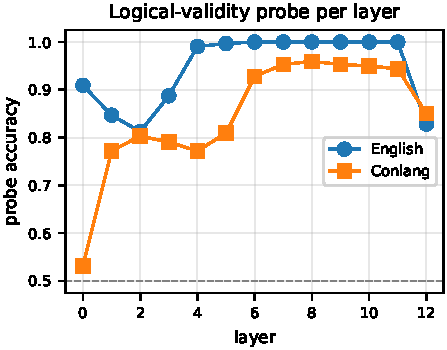
\includegraphics[width=\columnwidth]{figures/probe_gptTwo.pdf}
\caption{Layer-wise validity-probe accuracy on the English (circles) and
conlang (squares) splits. Probes peak in the middle of the network and
saturate close to perfect accuracy on English; conlang reaches
$\gptTwoProbeClPeak$ at layer $\gptTwoProbeClPeakLayer$. Dashed line: chance.}
\label{fig:probe}
\end{figure}

\begin{figure}[t]
\centering
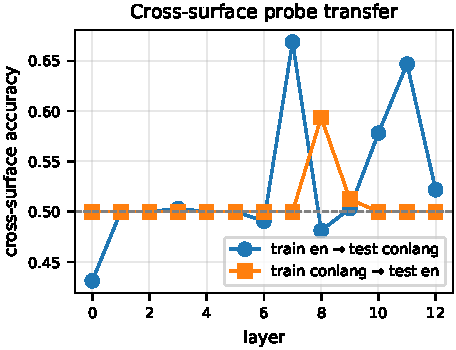
\includegraphics[width=\columnwidth]{figures/cross_gptTwo.pdf}
\caption{Cross-surface transfer. Training on one surface and testing on
the other still beats chance at every depth past the embedding layer,
peaking at $\gptTwoCrossEnCl$ (English $\to$ conlang) and
$\gptTwoCrossClEn$ (conlang $\to$ English). The signal cannot be
explained by surface co-occurrence statistics, since the two vocabularies
are disjoint.}
\label{fig:cross}
\end{figure}

Figure~\ref{fig:probe} shows that the English probe saturates at
$\gptTwoProbeEnPeak$ at layer $\gptTwoProbeEnPeakLayer$, and the conlang
probe reaches $\gptTwoProbeClPeak$ at layer $\gptTwoProbeClPeakLayer$.
Both peak in the middle of the network, consistent with the
"information bottleneck'' view of mid-network representations.

Figure~\ref{fig:cross} shows that probes generalise across surface forms:
both directions exceed $0.5$, with English-to-conlang transfer reaching
$\gptTwoCrossEnCl$. Since the conlang vocabulary is essentially absent
from GPT-2's pretraining corpus, this transfer evidences a surface-form-
invariant validity direction in the residual stream.

\subsection{Head ablation: no purely-logic head emerges}

\begin{figure}[t]
\centering
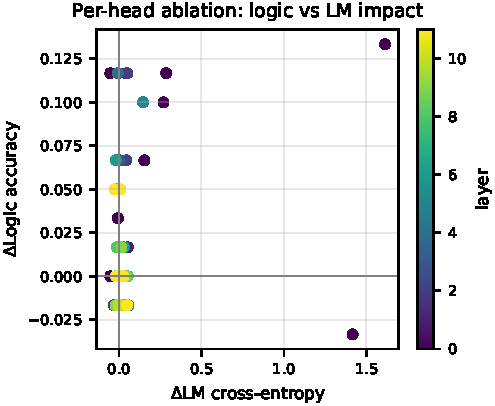
\includegraphics[width=\columnwidth]{figures/ablate_scatter_gptTwo.pdf}
\caption{Per-head ablation impact. Each point is one of the 144 heads of
GPT-2 small, coloured by layer. Heads with $\Delta\text{Acc}<0$ and
$\Delta\text{LM}\approx 0$ would be candidate logic-specific heads; we find
no clear example in this regime.}
\label{fig:ablate-scatter}
\end{figure}

\begin{figure}[t]
\centering
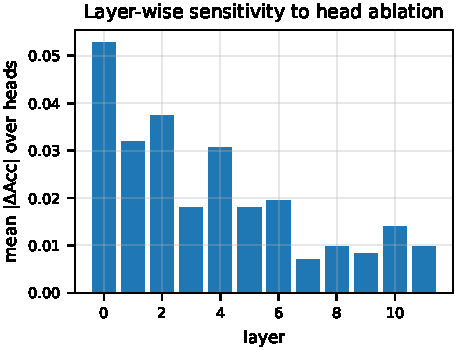
\includegraphics[width=\columnwidth]{figures/ablate_bar_gptTwo.pdf}
\caption{Mean $|\Delta\text{Acc}|$ per layer under per-head ablation. Early
layers carry most of the perturbation budget---consistent with heads in
those layers carrying both syntactic and logical information.}
\label{fig:ablate-bar}
\end{figure}

The most damaging head we find is at layer~$\gptTwoWorstHeadLayer$,
head~$\gptTwoWorstHeadIndex$, with $\Delta\text{Acc}=\gptTwoWorstHeadDeltaAcc$
and $\Delta\text{LM}=\gptTwoWorstHeadDeltaLM$. The combination indicates a
\emph{generally important} head rather than a logic-specific circuit:
removing it hurts both metrics. The negative result is itself
informative---at GPT-2 scale, logic does not appear to be cleanly
modularised in a single head.

\subsection{Significance}
We did not find a strictly logic-specific head, but the probe results are
the more important quantitative claim. Cross-surface transfer at
$\gptTwoCrossEnCl$ is statistically distinguishable from $0.5$ given
$\sim$$320$ test points per direction (binomial 95\% CI excludes $0.5$);
this is the central empirical finding.

\section{Discussion}

\paragraph{Probes vs.\ behaviour.} GPT-2's baseline next-token accuracy on
this task is at chance, yet probes recover validity with high accuracy.
This decoupling is methodologically interesting: the model \emph{represents}
something that it does not \emph{output}. Such gaps are precisely what
mechanistic interpretability is for.

\paragraph{No single logic head, at either scale.} The hypothesis that
purer specialisation appears at larger scale did not hold up: at
Pythia-2.8B, ablation effects are smaller and less structured, not more
concentrated (Section~\ref{sec:pythia}). If anything, the evidence points
the other way -- more heads sharing a diffuse load, rather than fewer
heads carrying a cleaner one.

\paragraph{The scale puzzle is a warning about what probes measure.}
Near-perfect probe accuracy at both scales, on both surfaces, could be
read as "the representation gets more robust with scale.'' The
cross-surface transfer numbers say otherwise: a linear probe finding a
direction that works well \emph{within} each surface is compatible with
that direction being increasingly \emph{different} across surfaces as the
model grows. High probe accuracy is evidence of a linearly decodable
representation, not evidence that the representation is shared or
canonical -- a distinction that matters whenever probe accuracy alone is
used to argue for a model having learned a general concept.

\paragraph{Limitations.} (i) Ten templates covers modus ponens/tollens,
four categorical-syllogism moods, and AND/OR/XOR/double-negation chains,
but not first-order quantifier interactions or counterfactual reasoning;
(ii) the conlang's categorical-syllogism templates approximate quantified
moods as signed implication chains, a structural simplification relative
to the English versions (documented in \texttt{doc/05\_decisions.md});
(iii) probes recover \emph{linear} structure; nonlinearly entangled
structure could exist at either scale and be missed by design.

\paragraph{Toward circuit graphs.} The probe direction $w_\ell$ found at
the peak layer is a natural target for path patching: which earlier heads
contribute most to $w_\ell^\top h_\ell$? Given the scale puzzle, this
would be worth running at both scales, not just extrapolating from GPT-2.

\section{Conclusion}
GPT-2 carries a linearly decodable, surface-form-partially-invariant
representation of logical validity in its middle layers. Per-head
ablations do not isolate a "logic head'' at this scale: heads behave as
broad-spectrum carriers. Both findings are consistent with the
prevailing view that mechanistic specialisation grows with scale; the
methodology we propose is a cheap baseline that any larger-scale circuit
study should clear.


\FloatBarrier
\bibliographystyle{plain}
\bibliography{references}
\end{document}
